\section{Exploratory Study}
Initial exploratory analysis aspects are provided in this section. Such studies and analysis resulted the methodologies utilized and experiment design. Initially Datasets from USRDS on CKD and ESRD patients were explored for Patient characteristics, prevelance of CKD, dietary intake, dietician care, mortality, and survival. Dietary intake data were missing though dietician care data, mortality and survival data by age groups were there; however, No linking data was there for dietician care data and target mortality and survival data. Hence, datasets from an study on dietary shift recommendation by CDC was explored where recommended intake amounts for each age groups including average intake amount (of food groups and food subgroups) by age groups  were provided.  However, Age groups between Dietary shift recommendation dataset and USRDS mortality i.e. target variable data were not aligned. Hence, dietary intake data from NHANES survey was explored. The same survey data was used by Dietary shift recommendation dataset. Hence, regrouped NHANES survey data to reflect the USRDS age groups. USDA codes wer used for Food groups/subgroups/intake food for NHANES survey. Hence, survey food intake was mapped using USDA food codes. Shift recommendation dataset along with additional data from CDC and other sources were explored to create food group recommended amounts for matching age groups. Initial exploratory analysis such as univariate analysis, bivariate analysis, Regression, and Factor analysis were done.  Representative exploratory analysis output and plots from the initial analysis are given in Figure \ref{exploratory-output}. However, the output and plots are primarily exploratory that may or may not reflect the final outcome. 

\begin{table}
\caption{\textbf{Regression Output from Exploratory Analysis using Excel (Data Analysis Module)}}
\begin{tabular}{  | p{7.5 cm} | p{7.5cm} | }
\hline
\textbf{Food Groups:}
Multiple R:	0.880156954, R Square:	0.774676264, Adjusted R Square: 	0.616949648, Standard Error:	6.223447127
&
\textbf{Food Subgroups:}
Multiple R:		0.999378722, R Square:		0.99875783,  Adjusted R Square:	 0.978883104, Standard Error:	1.461167293, Observations:		18, R Square: 99\% \\
\hline
\end{tabular}
\end{table}


\begin{figure}
\begin{tabular}{|c|}
\hline
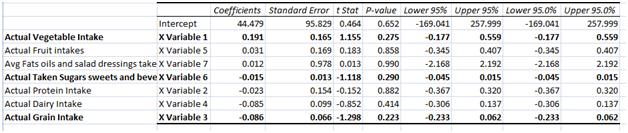
\includegraphics[scale=0.75]{excel-regression-food-groups} \\
\textbf{Regression on Actual Food Group Intake}\\
\hline
\end{tabular}

\begin{tabular}{|c|}
\hline
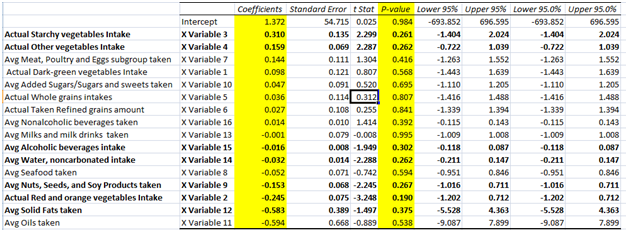
\includegraphics[scale=0.75]{excel-regression-food-subgroups}\\
\textbf{Regression on Actual Food Subgroup Intake} \\
\hline
\end{tabular}

\begin{tabular}{|c|}
\hline
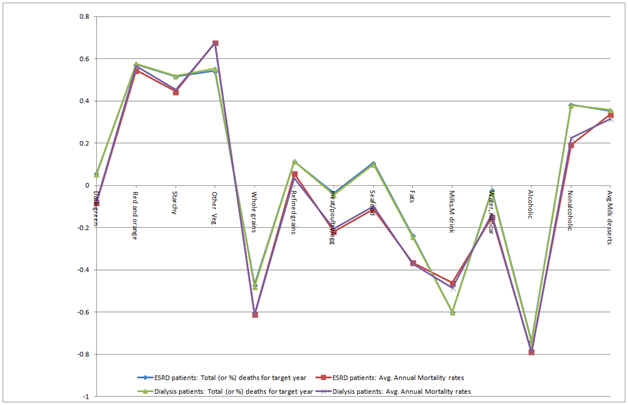
\includegraphics[scale=0.75]{line-plot-regression-exploratory.png}\\
\textbf{Line Plot for Regression outcome}\\
\hline
\end{tabular}

\begin{tabular}{|c|}
\hline
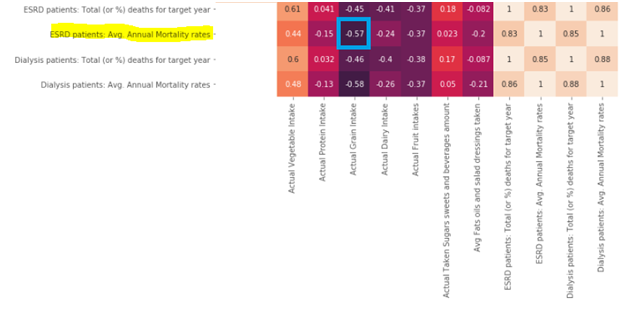
\includegraphics[scale=0.75]{heatmap-exploratory}\\
\textbf{Heatmap for exploration}\\
\hline
\end{tabular}
\caption{\textbf{Exploratory Analysis and Representative Output}}
\label{exploratory-output}
\end{figure}




